\documentclass[border=8pt]{standalone}
\usepackage{pgf-pie}
\usepackage{xcolor}

\definecolor{oasstcolor}{RGB}{52, 120, 190}
\definecolor{ultrachatcolor}{RGB}{34, 150, 100}
\definecolor{alpacacolor}{RGB}{190, 80, 50}
\definecolor{sharegptcolor}{RGB}{160, 100, 180}

\begin{document}
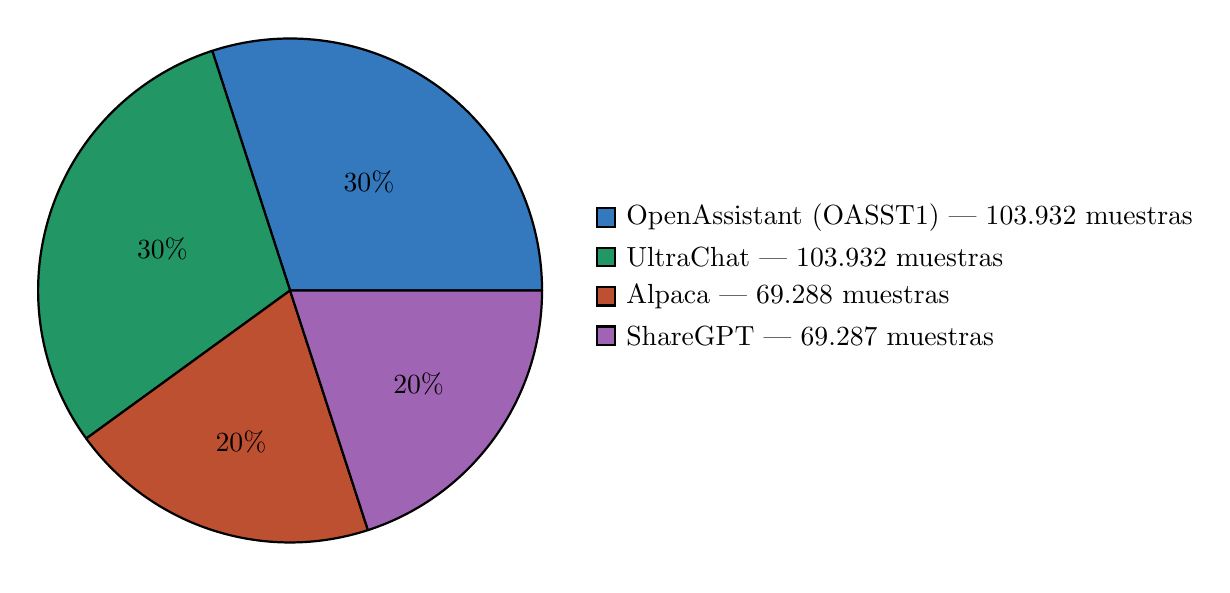
\begin{tikzpicture}
\pie[
    radius=3.2,
    color={oasstcolor, ultrachatcolor, alpacacolor, sharegptcolor},
    text=legend,
    after number=\%,
    every label/.style={font=\small}
]{
    30/OpenAssistant (OASST1) --- 103.932 muestras,
    30/UltraChat --- 103.932 muestras,
    20/Alpaca --- 69.288 muestras,
    20/ShareGPT --- 69.287 muestras
}
\end{tikzpicture}
\end{document}
